\documentclass[12pt]{jarticle}
\usepackage{TUSIReport}
\usepackage{bm}
\usepackage{ascmac}
\usepackage{framed}
\usepackage[dvipdfmx]{graphicx}
\begin{document}
\提出者{情報工学実験2}{実験テーマ1 数理計画法}{2020}{9}{21}{4619060}{照永詩恩}
\共同実験者{}{}{}{}{}{}{}{}
\表紙出力

\section{実験の原理(理論)}


\section{結果}
\begin{description}
	\item[(1)] 成人の食事問題については現実の最適化問題とみなせるのではないかという考えについた.この問題は,食品の種類をうまく決めて,
	      栄養バランスと成人が取るべき値である$1600[kcal]\sim 1800[kcal]$を制約条件として食品の量を最大化摂取するというものとみなせると考えた.
	\item[(2)]
	\item[問1]
	      2つの野菜の合計の値段を$f(\boldsymbol{x})$,2つの野菜のそれぞれの量を$x_1[g]$,$x_2[g]$,それぞれの単価を$c_1$,$c_2$,とする.
	      また,栄養素は$A_1$,$A_2$,$A_3$がある.栄養素$A_i$は一日$b_i[mg]$取らなければならない.ただし,$(i=1,2,3)$とする.この問題を定式化すると,
	      \begin{eqnarray}
		      f(\boldsymbol{x})=c_1 x_1 +c_2 x_2, \ S=\{\boldsymbol{x};x_1,x_2\in \boldsymbol{R},x_1,x_2\geq 1,a_{i1} x_i+a_{i2}x_i\geq b_i\}\nonumber
	      \end{eqnarray}
	      とすると,Minimize\ $f(\boldsymbol{x})$\ subject\ to \ $\boldsymbol{x}$ \ $\in$ $S$\ とかける.
	\item[問2] 野菜$V_1$の栄養素の定数を2,0.1,0.1とし$V_2$の定数を3,0.3,0.1とした.単価は0.1,0.15とした.
	      グラフを書きその端点をとってその中で一番値の小さいものを選んだ.結果は(1500,2000)が最適解となり,450が最適値となった.
	      \begin{center}
		      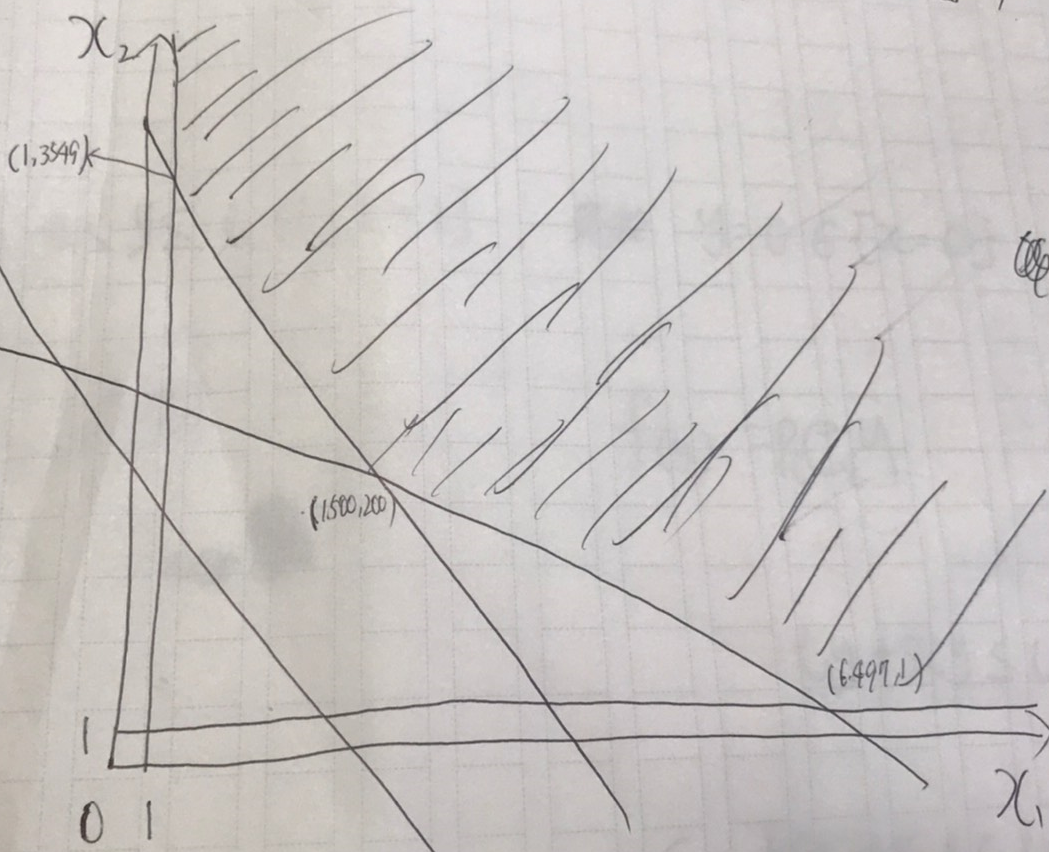
\includegraphics[height=4cm,width=6cm]{1.png}\\
		      図1:($x_1$,$x_2$)平面\\
	      \end{center}
	\item[問3]
	      300円以下で最大の嬉しさの値はチョコレートとクッキーとグミを買ったときの21となった. 
	\item[問4]
	\item[A]
	      $x_4$,$x_5$をそれぞれグミとガムとしてこの制約条件を数式化(線形式)で表すと,
	      \begin{eqnarray}
		      x_4+x_5<2\nonumber
	      \end{eqnarray}
	      とたてられることができる.
	\item[B]
	      $x_3$,$x_5$をそれぞれポテチとガムとしてこの制約条件を数式化すると
	      \begin{eqnarray}
		      x_3\leq x_5\nonumber
	      \end{eqnarray}
	\item[問5]
	      この条件を数式化するとそれぞれ
	      \begin{eqnarray}
		      a\leq y\leq b \in \{x=1\}\nonumber\\
		      y=0\in \{x=0\}\nonumber
	      \end{eqnarray}
	      となると考えた. 
	\item[問6]
	      稼働しているかしていないかという変数を$\boldsymbol{x}$(バイナリ変数),稼働時間を$\boldsymbol{y}$(連続変数)とおく.
	      $i=1,2$として目的関数,制約条件を次のように
	      \begin{eqnarray}
		      f(\boldsymbol{y})=p_ie_i\boldsymbol{y},\ \ S=\{\boldsymbol{y};a\leq y\leq b\in \{\boldsymbol{x}=1\},y=0\in \{\boldsymbol{x}=0\},t_iy+s_iy\leq U\}
	      \end{eqnarray}
	      として,Maximize \ $f(x)$ \ subject\ to\ $\boldsymbol{y}\in$ S とかく.
	\item[(3)]
	      「とある学校で6科目中3科目のテストを受けなければいけない.事前にそれぞれの科目はどのくらい得意なのかというアンケートを取りさらに
	      問題作成者に難易度はどれくらいかを聞いたという設定にする.Aくんは難易度が150を超えてしまうと精神状態が悪くなり今までの力が発揮できなくなってしまうようです.
	      それ以下であれば得意であれば得意であるほど点数が高くなるようです.どの科目を選ぶのが最適でアンケートで答えた数値の合計はいくつになるか」という問題を作成した.
	      \begin{table}[h]
		      \caption{Aくんがそれぞれどれくらい得意なのかとその科目のテストの難易度}
		      \begin{center}
			      \begin{tabular}{|c|c|c|c|c|c|c|}
				      \hline
				                   & $x_1$ & $x_2$ & $x_3$ & $x_4$ & $x_5$ & $x_6$ \\
				      \hline
				      得意の度合い & 10    & 8     & 9     & 4     & 5     & 1     \\
				      \hline
				      難易度       & 80    & 60    & 70    & 50    & 40    & 10    \\
				      \hline
			      \end{tabular}
		      \end{center}
	      \end{table}
	      これを定式化してみる.\\
	      決定変数は受けるか受けないかということでバイナリ変数$\boldsymbol{x}$とする.目的関数と制約条件をそれぞれ,
	      \begin{eqnarray}
		      f(\boldsymbol{x})&=&10x_1+8x_2+9x_3+4x_4+5x_5+x_6\nonumber\\
		      S&=&\{\boldsymbol{x};x_1,x_2,x_3,x_4,x_5,x_6\in \{0,1\},\nonumber\\
		      &&x_1+x_2+x_3+x_4+x_5+x_6=3,\nonumber\\
		      &&80x_1+60x_2+70x_3+50x_4+40x_5+10x_6\leq 150\}\nonumber
	      \end{eqnarray}
	      と書くことができ,Maximize \ $f(x)$ \ subject\ to\ $\boldsymbol{y}\in$ S とかく.       
\end{description}
\section{検討・考察}
\begin{description}
	\item[(2)]
	\item[問1] この問題は値段の合計を最適化するのでそれを目的関数,決定変数を野菜の量にした.
	      決定した目的関数と決定変数を利用して値段の合計を求める式と制約条件の式を設定することが
	      できると考えた.
	\item[問2]
	      グラフで領域を書いて端点のどれかが最適解だと考えた.今回の自ら設定した定数の場合端点は3つ出てきたので
	      それぞれの端点を代入して最小値をだしてそれを最適値とした. 
	\item[問3]
	      全$2^5=32$通りを探索するという考えでC言語を用いた.
	      配列(嬉しさ,値段,$0\sim 32$の二進数各ビット格納)とfor文,各ビットの論理積を使って最適値をだした.
	      また,最適値がでたときの組み合わせとして10進数表記で出力される.それを2進数変換することで組み合わせ
	      を求めることができると考えた. 
	\item[問4]
	      ポテチとガムの両方を買うことはできなくバイナリ変数を使っていることからこの場合$x_4+x_5=2$となる.
	      つまりこれ以外のものになればよいというものでありかつ$x_4+x_5$の最大値は2でありしかも両方買うという場合の値のみなので
	      結果のような式を立てた.\\
	      ポテチを買うならガムを買うという条件に対して,ポテチを買うがガムを買わないということはしてはいけない.
	      これらの決定変数は0か1が答えでありこの条件が当てはまるものとして$x_3=x_5$もしくは$x_3<x_5$ということになるのではないかと考えた.   
	\item[問5]
	      これらの条件を$\{x=0\}$という集合の中に含んでいる,$\{x=1\}$の集合に含んでいると書くことで表現できるのではないかと考えた.   
	\item[問6]
	      問5で数式化したものも使い稼働時間を決定変数$\boldsymbol{y}$として総利益を最大にする目的なので総利益を目的関数とした.
	      稼働しているとき一日の総消費電力が制約条件に入っていたのでセットアップに使う電力と単位時間に使う電力を決定変数を利用して数式化することで
	      正しい定式化ができるのではないかと考えた. 
	\item[(3)]
	      バイナリ変数を決定変数とする問題を作成してみた.私自身も一般教養を選択するにおいて前年度の成績の比率などを参考にしている.そのような経験から
	      このような問題を作る発想に至った.  
\end{description}
\section{結論}
例題を通して定式化する方法を身に着けることができた.また,その簡単な例題から最適値を求めることができた.
\begin{thebibliography}{99}
	\label{sannkoubunnkenn_chapter}
	\bibitem{rikadai}
	情報工学実験1,
	東京理科大学 工学部 情報工学科, 2020. 
\end{thebibliography}
\clearpage
% 付録
\appendix
\section{付録}
\begin{framed}
	\begin{verbatim}
#include<stdio.h>
int main()
{
	int a[5]={10,5,7,6,3};//嬉しさ
	int b[5]={140,80,130,70,30};//値段
	int c=1;//論理積につかう値
	int d[32][5];//各セルに対して0か1を格納するための配列
	int i,j;//for文に使う
	int k;//論理積の結果を代入する用
	int ans1,ans2;//嬉しさと値段の合計
	int e=-100000000,f=300;//嬉しさの最大値と制約条件である300円
	int g;//10進数表記用
			
	for(i=0;i<32;i++)//配列dに1~32までの二進数の各ビットの数字を格納
	{
		k=i+1;
		for(j=4;j>=0;j--)
		{
			d[i][j]=k&c;
			k=k >> 1;
		}
	}
			
	for(i=0;i<32;i++)//嬉しさと値段の合計を求めて最適値を出す
	{
		ans1=0;
		ans2=0;
		for(j=0;j<5;j++)
		{
 			ans1+=a[j]*d[i][j];
			ans2+=b[j]*d[i][j];
		}
		if(ans1>e&&ans2<=f&&ans1>0)
		{
			e=ans1;
			g=i+1;
		}
	}
			
	printf("最適値%d(%dのとき)\n",e,g);
	return 0;
}
    \end{verbatim}
\end{framed}
\begin{center}
	図A.2:(2)の問3ソースコード
\end{center}
\end{document}